\documentclass[oneside]{Ontario_Tech_Thesis}

\usepackage{lipsum} % Only for the sample

% Thesis properties
\title{Your Thesis Title}
\date{\today}
\author{Your Name}
\degree{Your Degree}
\faculty{Your Faculty}
\program{Your Program}
% By default the university is UOIT, this can be changed by uncommenting the following 
%\university{Your University}
%\city{Your city and country}

% Defense properties
\defense{July 1, 2019}
\chair{Thesis Chair}
\supervisor{Your Supervisor}
\committee{Committee Member 1}{Committee Member 2}
\examiner{External Examiner, Their Affiliation} % Thesis / External Examiner
%\univexaminer{} % University Examiner (PhD Only)

\begin{document}
\pagenumbering{roman} 
\maketitle

\makeexaminfo

\makeabstract{
Put your abstract here.
}

\makeacknowledgements{
Thank some people that you like here.
}

\makedeclaration

\makecontributions{
The work described in Chapter \ref{chap:chap2} was performed at the Futuristic Automotive Research Centre of Excellence (FARCE) in Hill Valley, California, using the Flux Capacitor testing laboratory operated by Dr. Emmett Brown. I was responsible for installing and testing flux capacitors in my automotive prototype vehicles.
}

{\hypersetup{linkcolor=black}
\maketableofcontents
}

\pagenumbering{arabic}
\doublespacing

\chapter{First Chapter Title}
\lipsum[1-2]
\section{First Section}
\lipsum[3-4]

\chapter{Second Chapter Title}
\label{chap:chap2}
\lipsum[5-6]
\begin{figure}[tbp]
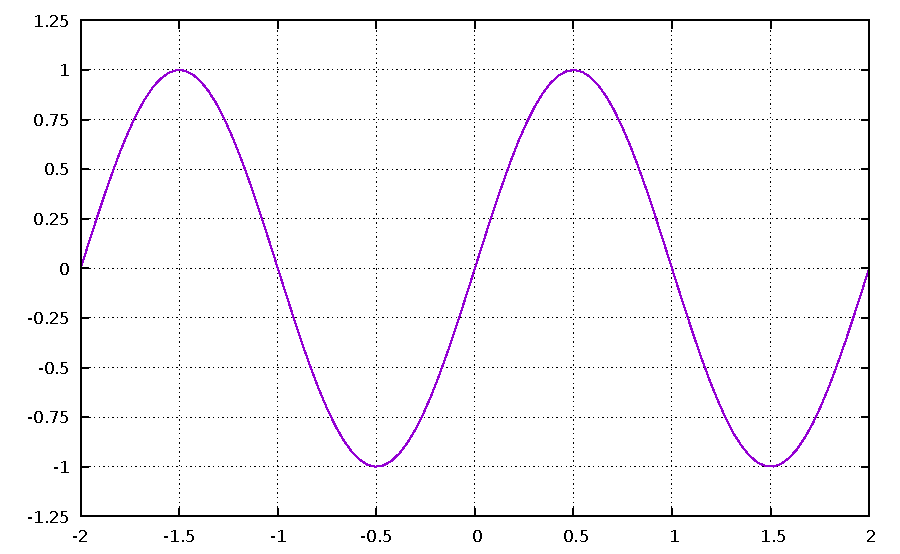
\includegraphics{Plot}
\caption{Beautiful plot of $y = \sin(\pi x)$.}
\end{figure}
\lipsum[7-8]

% Adds references to table of contents
\phantomsection 
\addcontentsline{toc}{chapter}{References} 

\nocite{*} % Only for the sample
\bibliography{Ref}

\appendix

\chapter{Sample Appendix}
\lipsum[9-12]

\end{document}
